\documentclass{beamer}
\usetheme{Madrid}

\usepackage{amsmath, amssymb, amsthm}
\usepackage{graphicx}
\usepackage{listings}
\usepackage[utf8]{inputenc}
\usepackage{hyperref}

\title{11.16.3.7}
\author{EE24BTECH11004 - Ankit Jainar}
\date{\today}

\begin{document}

\frame{\titlepage}

\begin{frame}
\frametitle{Question}
Three coins are tossed once. Find the probability of getting exactly two tails.
\end{frame}
\begin{frame}
\frametitle{Theoretical Solution}
The sample space for tossing three coins is:
\[
S = \{HHH, HHT, HTH, HTT, THH, THT, TTH, TTT\}.
\]
The total number of outcomes is:
\[
|S| = 8.
\]
The favorable outcomes for exactly two tails are:
\[
A = \{HTT, THT, TTH\}.
\]
The number of favorable outcomes is:
\[
|A| = 3.
\]
The probability of getting exactly two tails is:
\[
P(A) = \frac{|A|}{|S|} = \frac{3}{8} = 0.375.
\]
\end{frame}

\begin{frame}
\frametitle{Introduction}
This task involves simulating the random tossing of three coins using a C program, compiling it into a shared object (.so)file and using Python to process the results and generate a Probability Distribution plot, Probability Mass Function, Cumulative Distribution Function.
\end{frame}
\begin{frame}
\frametitle{C Code Description}
The C program generates random samples for the coin tosses, where the outcomes are categorized based on the number of tails. The program uses the \texttt{rand()} function to simulate the random tosses and increments a counter for each outcome with exactly two tails.
\end{frame}
\begin{frame}{Python Code Description}
    The Python code performs the following:
\begin{enumerate}
    \item Loads the shared object file generated from the C program using the \texttt{ctypes} library.
    \item Simulates a specified number of random coin tosses (e.g., 1,000,000 trials).
    \item Calculates the probability of getting exactly two tails using the formula:
    \begin{align}
    P(\text{exactly two tails}) = \frac{\text{frequency of exactly two tails}}{\text{total trials}}
    \end{align}
    \item Plots the probability distribution,mass and cumulative distribution functions using \texttt{matplotlib}.
\end{enumerate}

\end{frame}

\begin{frame}
\frametitle{Graphical Output}
The Python code generates a bar chart where:
\begin{itemize}
    \item The x-axis represents the outcomes: "0 tails", "1 tail", "2 tails", and "3 tails".
    \item The y-axis represents the probabilities, ranging from 0 to 1.
    \item The bar height for "2 tails" corresponds to the probability \(P(A) = 0.375\).
\end{itemize}
\end{frame}

\begin{frame}
\frametitle{Probability Mass Function (PMF)}
The PMF represents the probability of each individual outcome in the sample space \(S\). For the coin toss:
\[
S = \{0 \text{ tails}, 1 \text{ tail}, 2 \text{ tails}, 3 \text{ tails}\}.
\]
The PMF is given as:
\[
P(X = x) = 
\begin{cases} 
\frac{1}{8}, & x = 0 \text{ tails}, \\
\frac{3}{8}, & x = 1 \text{ tail}, \\
\frac{3}{8}, & x = 2 \text{ tails}, \\
\frac{1}{8}, & x = 3 \text{ tails}.
\end{cases}
\]
\end{frame}

\begin{frame}
\frametitle{Cumulative Distribution Function (CDF)}
The CDF represents the cumulative probability of outcomes up to a given value \(x\), defined as:
\[
F(x) = P(X \leq x) = \sum_{k \in S, k \leq x} P(X = k).
\]
For the coin toss:
\[
F(x) = 
\begin{cases} 
0, & x < 0, \\
\frac{1}{8}, & x = 0, \\
\frac{4}{8}, & x = 1, \\
\frac{7}{8}, & x = 2, \\
1, & x \geq 3.
\end{cases}
\]
\end{frame}

\begin{frame}
\frametitle{Simulation Process}
We simulate the tossing of three coins using the following steps:
\begin{enumerate}
    \item The sample space consists of outcomes in the set:
    \[
    S = \{0 \text{ tails}, 1 \text{ tail}, 2 \text{ tails}, 3 \text{ tails}\}.
    \]
    \item For each simulated toss, a random integer \(X\) is generated such that:
    \[
    X \in \{0, 1, 2, 3\},
    \]
    using a random number generator function based on binomial trials.
    \item The number of occurrences of each outcome is tracked over \(N\) trials, where \(N\) is the total number of simulations.
    \item Both the PMF and CDF are computed:
    \begin{itemize}
        \item \textbf{PMF}: The frquency of each outcome is divided by the total number of trials to compute the probabilities.
        \item \textbf{CDF}: The cumulative probabilities are calculated as the running total of the PMF values.
    \end{itemize}
\end{enumerate}
\end{frame}

\begin{frame}
\frametitle{Conclusion}
This task demonstrates the integration of C and Python for simulating and visualizing a probabilistic experiment. The probability of getting exactly two tails from tossing three coins is calculated as \textbf{0.375}, matching the theoretical value.
\end{frame}

\begin{frame}
\frametitle{Graphical Results}

\begin{figure}[h!]
   \centering
   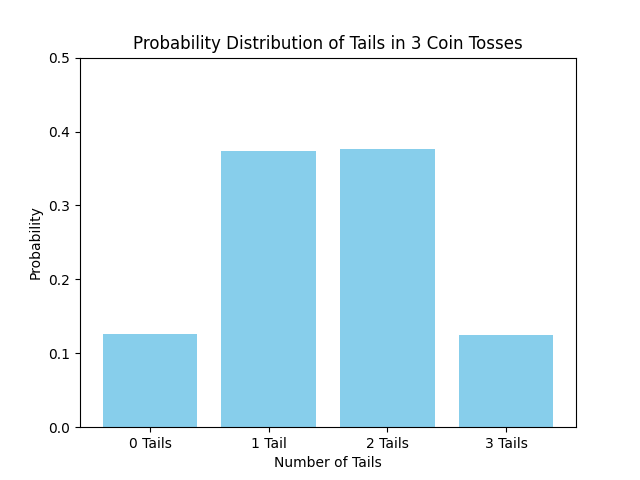
\includegraphics[width=0.7\linewidth]{figs/fig1.png}
   \caption{Probability Distributive Function (PDF)}
\end{figure}
\end{frame}
\begin{figure}[h!]
   \centering
   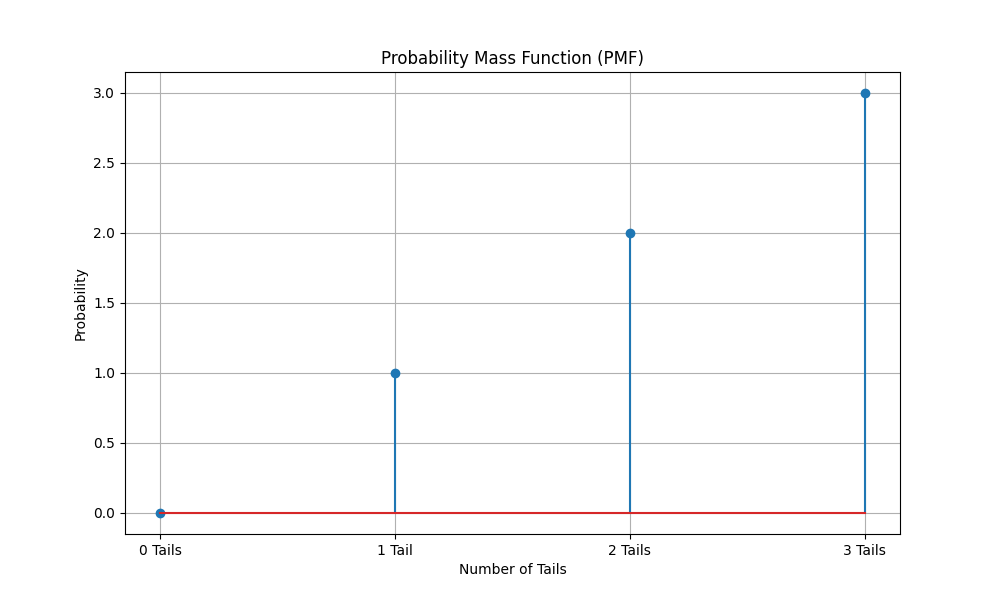
\includegraphics[width=0.7\linewidth]{figs/fig2.png}
   \caption{Probability Mass Function (PMF)}
\end{figure}
\end{frame}
\begin{figure}[h!]
   \centering
   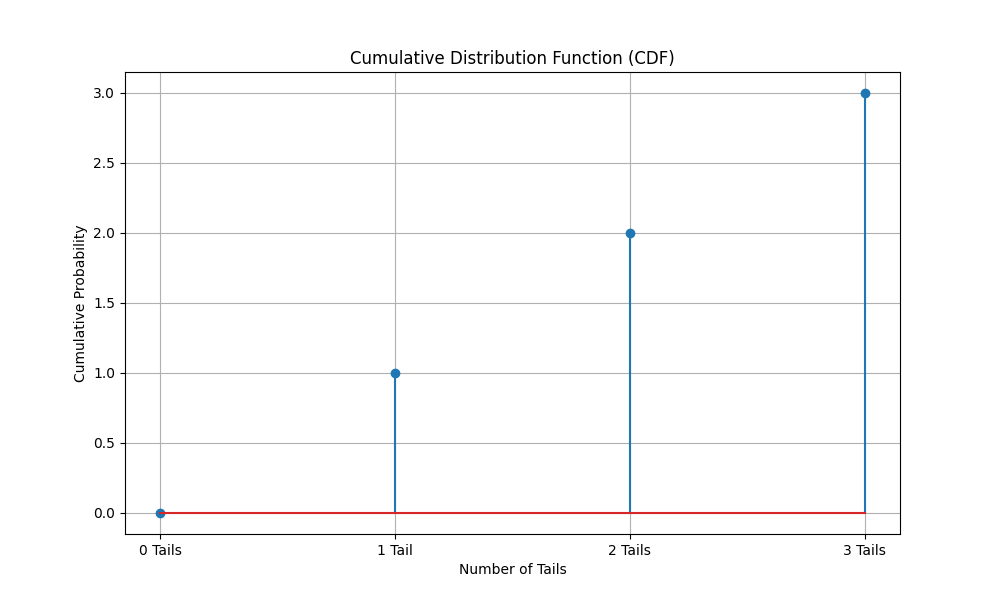
\includegraphics[width=0.7\linewidth]{figs/fig3.png}
   \caption{Cumulative Distribution Function (CDF)}
\end{figure}
\end{frame}


\end{document}
